% Figure 7, narrow screens. From offer to answer. Labels: LABELS.md, Figure 7.
% Same text and crimson focus as fig7-offer-timeline.tex, stacked for a phone. Width matches fig1 narrow.
\def\eeprepfigure{1}
\providecommand{\eepstyledir}{../style}% repo: ../style
\input{\eepstyledir/circuitikz-preamble.tex}
% Colours, fonts, and text styles for the Get hired figures.
% Input after style/circuitikz-preamble.tex (in the repo: ../../style/circuitikz-preamble.tex).
% Define \eepdark before this file for the dark build. Same names as the resume figures,
% plus the rest of the navy palette. Crimson (eepaccent) marks one thing per figure.
\setmainfont{Newsreader}[
  BoldFont={Newsreader Bold},
  ItalicFont={Newsreader Italic},
  BoldItalicFont={Newsreader Bold Italic},
]
\usetikzlibrary{arrows.meta,calc,decorations.pathreplacing}
\ifdefined\eepdark
  \definecolor{eepink}{HTML}{ECEEF2}
  \definecolor{eeptext}{HTML}{D0D4DB}
  \definecolor{eepinktwo}{HTML}{A6AFBF}
  \definecolor{eepmute}{HTML}{8F95A0}
  \definecolor{eepsilver}{HTML}{76808F}
  \definecolor{eeprule}{HTML}{3B4352}
  \definecolor{eepwash}{HTML}{17243A}
  \definecolor{eepsunken}{HTML}{101828}
  \definecolor{eepfill}{HTML}{131C2E}
  \definecolor{eeppaper}{HTML}{0D1524}
  \definecolor{eepaccent}{HTML}{E06A5F}
  \definecolor{eepaccentsoft}{HTML}{2A1A24}
\else
  \definecolor{eepink}{HTML}{16233A}
  \definecolor{eeptext}{HTML}{232A39}
  \definecolor{eepinktwo}{HTML}{424D63}
  \definecolor{eepmute}{HTML}{5E636C}
  \definecolor{eepsilver}{HTML}{838C9A}
  \definecolor{eeprule}{HTML}{C4C8CF}
  \definecolor{eepwash}{HTML}{E7ECF3}
  \definecolor{eepsunken}{HTML}{F3F4F6}
  \definecolor{eepfill}{HTML}{FFFFFF}
  \definecolor{eeppaper}{HTML}{FBFBFC}
  \definecolor{eepaccent}{HTML}{A3201D}
  \definecolor{eepaccentsoft}{HTML}{F8ECEA}
\fi
% Draw in y-down points so coordinates read like a mockup: [x=1pt, y=-1pt].
\tikzset{
  eeptitle/.style={anchor=base west, inner sep=0pt, text=eepink, font=\rmfamily\bfseries\fontsize{26}{31}\selectfont},
  eephead/.style={inner sep=0pt, text=eepink, font=\sffamily\bfseries\fontsize{14.5}{18}\selectfont},
  eepbody/.style={inner sep=0pt, text=eepinktwo, font=\sffamily\fontsize{13}{17}\selectfont},
  eepnote/.style={inner sep=0pt, text=eepmute, font=\sffamily\fontsize{12.5}{16}\selectfont},
  eepsrc/.style={anchor=north west, inner sep=0pt, align=left, text=eepmute, font=\sffamily\fontsize{11}{14.5}\selectfont},
  eepbox/.style={draw=eepink, fill=eepfill, rounded corners=4pt},
  eepfocus/.style={draw=eepaccent, fill=eepfill, rounded corners=4pt, line width=1.8pt},
  eeparrow/.style={-{Stealth[length=8pt,width=6pt]}},
  eepdash/.style={dash pattern=on 4pt off 4pt},
  eeplead/.style={draw=eepsilver, line width=0.9pt},
}
% A dot on a trace, like a schematic junction.
\newcommand{\eepdot}[2][eepink]{\fill[#1] #2 circle (3.6pt);}
% Short labels never hyphenate.
\hyphenpenalty=10000 \exhyphenpenalty=10000
% One space after a full stop, as on the site.
\frenchspacing

% #1 name, #2 previous node, #3 text. The dot sits on the trace at x = 40.
\newcommand{\offerstep}[3]{%
  \node[eepbody, text=eepink, anchor=north west, text width=290pt, align=left] (#1) at ($(#2.south west)+(0,22)$) {#3};
  \eepdot{($(#1.north west)+(-24,8)$)}}
\begin{document}
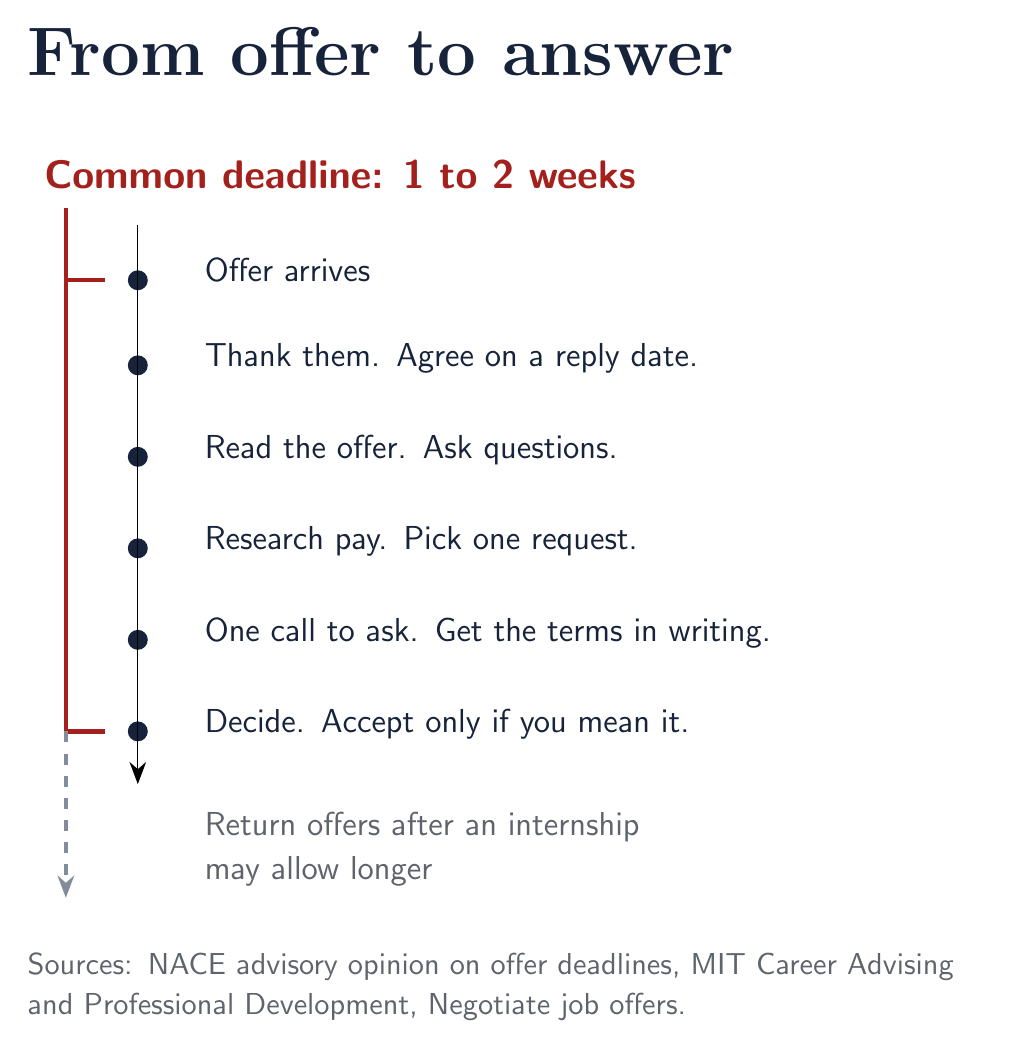
\begin{tikzpicture}[x=1pt,y=-1pt]
  \node[eeptitle] at (0,30) {From offer to answer};
  \node[eephead, text=eepaccent, anchor=west] at (6,66) {Common deadline: 1 to 2 weeks};
  \coordinate (s0) at (64,74);
  \offerstep{s1}{s0}{Offer arrives}
  \offerstep{s2}{s1}{Thank them. Agree on a reply date.}
  \offerstep{s3}{s2}{Read the offer. Ask questions.}
  \offerstep{s4}{s3}{Research pay. Pick one request.}
  \offerstep{s5}{s4}{One call to ask. Get the terms in writing.}
  \offerstep{s6}{s5}{Decide. Accept only if you mean it.}
  \node[eepnote, anchor=north west, text width=290pt, align=left] (ext) at ($(s6.south west)+(0,26)$) {Return offers after an internship\\ may allow longer};
  % The trace, behind the step dots.
  \draw[eeparrow] ($(s1.north west)+(-24,-12)$) -- ($(s6.south west)+(-24,16)$);
  % Bracket from step 1 to step 6, read from the label above it, like a timing spec.
  \draw[eepaccent, line width=1.6pt] (14,78) -- ($(s6.north west)+(-50,8)$) -- ($(s6.north west)+(-36,8)$);
  \draw[eepaccent, line width=1.6pt] ($(s1.north west)+(-50,8)$) -- ($(s1.north west)+(-36,8)$);
  % Dashed extension for return offers.
  \draw[eepsilver, line width=1.3pt, eepdash, eeparrow] ($(s6.north west)+(-50,8)$) -- ($(ext.south west)+(-50,4)$);
  \node[eepsrc, text width=354pt] at ($(ext.south west)+(-64,24)$) {Sources: NACE advisory opinion on offer deadlines, MIT Career Advising and Professional Development, Negotiate job offers.};
\end{tikzpicture}
\end{document}
